% %%%%%%%%%%%%%%%%%%%%%%%%%%%%%%%%%%%%%%%%%%%%%%%%%%%%%%%%%%%%%%%%%%%%%%%%%%%%%
% thesis.tex: Primary TeX control file for thesis.
% %%%%%%%%%%%%%%%%%%%%%%%%%%%%%%%%%%%%%%%%%%%%%%%%%%%%%%%%%%%%%%%%%%%%%%%%%%%%%
\documentclass[11pt, oneside]{mnthesis}
\usepackage{epsfig} % Allows the inclusion of eps files
\usepackage{epic} % Enhanced picture mode
\usepackage{eepic} % Extensions for epic
\usepackage{units} % SI unit typesetting
\usepackage{url} % URL handling
\usepackage{longtable} % Tables that continue onto multiple pages
\usepackage{mathrsfs} % Support for \mathscr script
\usepackage{multirow} % Span rows in tables
\usepackage{bigstrut} % Space struts in tables up and down
\usepackage{amssymb} % AMS math symbols and helpers
\usepackage{graphicx} % Enhanced graphics support
\usepackage{setspace} % Adjust spacing in captions, single by default
\usepackage{xspace} % Automatically adjusting space after macros
\usepackage{amsmath} % \text, and other math formatting options
\usepackage{siunitx} % \num{} formatting and SI unit formatting
\usepackage{booktabs} % Enhanced tables with \toprule, etc.
\usepackage{hyperref} % Add clickable links to other parts of the document
\usepackage[noabbrev]{cleveref} % Automatically determine \cref type

\usepackage{parskip} % http://ctan.org/pkg/parskip


% Configure the siunitx package
\sisetup{
    group-separator = {,}, % Use , to separate groups of digits, like 12,345
    list-final-separator = {, and } % Always use the serial comma in \SIlist
}

% Configure the cleveref package
\newcommand{\creflastconjunction}{, and } % Always use the serial comma




% Names with special characters. 
\newcommand{\Alfven}{Alfv\'en\xspace}
\newcommand{\Ampere}{Amp\`ere\xspace}

% To make sure the capitalization is consistent. 
\newcommand{\ohmlaw}{Ohm's Law\xspace}
\newcommand{\amplaw}{\Ampere's Law\xspace}
\newcommand{\farlaw}{Faraday's Law\xspace}

% Field-aligned unit vectors. 
\newcommand{\xhat}{\ensuremath{\hat{x}}\xspace}
\newcommand{\yhat}{\ensuremath{\hat{y}}\xspace}
\newcommand{\zhat}{\ensuremath{\hat{z}}\xspace}

% Spherical unit vectors. 
\newcommand{\rhat}{\ensuremath{\hat{r}}\xspace}
\newcommand{\qhat}{\ensuremath{\hat{\theta}}\xspace}
\newcommand{\fhat}{\ensuremath{\hat{\phi}}\xspace}

% Use underlines for vectors and tensors. 
\renewcommand{\vec}[1]{\underline{#1}}
\newcommand{\tensor}[1]{\underline{\underline{#1}}}

% Differential operators. 
\newcommand{\dd}[1]{\ensuremath{ \frac{\partial}{\partial #1} }\xspace}
\newcommand{\ddt}{\dd{t}\xspace}
\newcommand{\curl}[1]{\ensuremath{ \nabla \times \vec{#1} }\xspace}
\renewcommand{\div}[1]{\ensuremath{ \nabla \cdot \vec{#1} }\xspace}
\newcommand{\grad}[1]{\ensuremath{ \nabla #1 }\xspace}

% Properly-scaled parentheses for grouping terms or for arguments. 
\newcommand{\lr}[1]{ \left( #1 \right) }
\newcommand{\lrsmall}[1]{ \left( {\scriptstyle #1} \right) }
\renewcommand{\arg}[1]{\!\lr{#1}}
\newcommand{\argsmall}[1]{\!\lrsmall{#1}}
\newcommand{\lrb}[1]{ \left[ #1 \right] }

% Circled plus-minus symbol. Solving quartics requires \pm and \opm. 
\newcommand{\opm}{ \text{ \textcircled{ \ensuremath{\hskip -0.2em \pm} } } \xspace}

% Define a better looking eV by moving the V slightly left
\DeclareSIUnit\electronvolt{e\hspace{-0.08em}V}

\DeclareSIUnit\RE{R_E}


\newcommand{\dt}{\ensuremath{\delta \hspace{-0.1em} t} \xspace}



% Azimuthal modenumber, typically indicated with a lowercase m. 
\newcommand{\azm}{\ensuremath{m_{azimuthal}}\xspace}

% Azimuthal modenumber, typically indicated with a lowercase m. 
\newcommand{\me}{\ensuremath{m_{e}}\xspace}

% Jacobian dererminant, typically indicated with a capital J, which we are using for current. 
\newcommand{\jac}{\ensuremath{D}\xspace}

% Dispersion tensor, typically indicated with... a capital D?
\newcommand{\dispersiontensor}{\tensor{T}\xspace}


% These things just get used a lot in the dispersion relation chapter...

% Boris-corrected speed of light. 
\newcommand{\cb}{\ensuremath{c_B} \xspace}

% Boris-corrected plasma frequency. 
\newcommand{\ob}{\ensuremath{\omega_B} \xspace}

% Boris-corrected electric constant. 
\newcommand{\eb}{\ensuremath{\epsilon_B} \xspace}

% Alfven speed. 
\newcommand{\va}{\ensuremath{v_A} \xspace}

% Perpendicular electric constant. 
\newcommand{\ep}{\ensuremath{\epsilon_\bot} \xspace}

% Epsilon zero. 
\newcommand{\ez}{\ensuremath{\epsilon_0} \xspace}

% Conductivities. 
\newcommand{\sz}{\ensuremath{\sigma_0} \xspace}
\newcommand{\sh}{\ensuremath{\sigma_H} \xspace}
\renewcommand{\sp}{\ensuremath{\sigma_P} \xspace}




\newcommand{\spe}{\ensuremath{\frac{\sigma_P}{\ep}} \xspace}
\newcommand{\she}{\ensuremath{\frac{\sigma_H}{\ep}} \xspace}




% 3x3 matrix. 
\newcommand{\mmm}[9]{ \left[ \begin{array}{ccc}
    #1 & #2 & #3 \\
    #4 & #5 & #6 \\
    #7 & #8 & #9
  \end{array} \right] }

% 2x2 matrix. 
\newcommand{\mm}[4]{ \left[ \begin{array}{cc}
    #1 & #2 \\
    #3 & #4
  \end{array} \right] }

% 2x1 matrix, or 2-vector. 
\newcommand{\vv}[2]{ \left[ \begin{array}{c}
    #1 \\
    #2
  \end{array} \right] }


% Physics constants
\newcommand{\C}{{\mathrm{c}}}

% Add space between rows of tables
\newcommand{\spacerows}[1]{\renewcommand{\arraystretch}{#1}}









\linespread{1.3}

% Compile only the chapters listed here. This may make the compile faster, but
% it's not necessary. 
%\includeonly{
%    preliminaries/title,
%    chapters/intro,
%    chapters/model,
%    chapters/math,
%    chapters/results,
%    chapters/data,
%    chapters/conclusion,
%    chapters/app_geometry,
%    chapters/app_integrating,
%}



% %%%%%%%%%%%%%%%%%%%%%%%%%%%%%%%%%%%%%%%%%%%%%%%%%%%%%%%%%%%%%%%%%%%%%%%%%%%%%
% %%%%%%%%%%%%%%%%%%%%%%%%%%%%%%%%%%%%%%%%%%%%%%%%%%%%%%% Mark this as a draft. 
% %%%%%%%%%%%%%%%%%%%%%%%%%%%%%%%%%%%%%%%%%%%%%%%%%%%%%%%%%%%%%%%%%%%%%%%%%%%%%
\draft
% %%%%%%%%%%%%%%%%%%%%%%%%%%%%%%%%%%%%%%%%%%%%%%%%%%%%%%%%%%%%%%%%%%%%%%%%%%%%%
% %%%%%%%%%%%%%%%%%%%%%%%%%%%%%%%%%%%%%%%%%%%%%%%%%%%%%%%%%%%%%%%%%%%%%%%%%%%%%
% %%%%%%%%%%%%%%%%%%%%%%%%%%%%%%%%%%%%%%%%%%%%%%%%%%%%%%%%%%%%%%%%%%%%%%%%%%%%%






\begin{document}
\bibliographystyle{hunsrt} % style of bibliography

% Title and other sections that come before the body of the document
%%%%%%%%%%%%%%%%%%%%%%%%%%%%%%%%%%%%%%%%%%%%%%%%%%%%%%%%%%%%%%%%%%%%%%%%%%%%%%%%
% title.tex - Set up the beginning of thesis.
%%%%%%%%%%%%%%%%%%%%%%%%%%%%%%%%%%%%%%%%%%%%%%%%%%%%%%%%%%%%%%%%%%%%%%%%%%%%%%%%

% Uncomment to turn on draft mode, which changes the title page to have a draft
% label and date of compilation
%\draft

% Set the type of thesis
\phd % use if for a Ph.D. dissertation
%\ms % use if for a Master of Science thesis

% Set the title and your name. Remember that the guidelines state:
%
% "The title of the thesis must not contain chemical or mathematical formulas,
% symbols, superscripts, subscripts, Greek letters, or other non-standard
% characters; words must be substituted."
\title{\bf Modeling Current-Driven Pc4 Pulsations in Two and a Half Dimensions}
\author{Charles A McEachern}
% Advisor name, put co-advisors here as well separated by commas
\director{Robert L Lysak}

% Specify the month and year; if commented out then these default to the
% current month and year
\submissionmonth{April}
\submissionyear{2016}

% Pages after the title page
\abstract{% %%%%%%%%%%%%%%%%%%%%%%%%%%%%%%%%%%%%%%%%%%%%%%%%%%%%%%%%%%%%%%%%%%%%%%%%%%%%%
% %%%%%%%%%%%%%%%%%%%%%%%%%%%%%%%%%%%%%%%%%%%%%%%%%%%%%%%%%%%%%%%%%%%% Abstract
% %%%%%%%%%%%%%%%%%%%%%%%%%%%%%%%%%%%%%%%%%%%%%%%%%%%%%%%%%%%%%%%%%%%%%%%%%%%%%

Abstract placeholder. 
}
\copyrightpage % Do you want copyright protection?
\acknowledgements{%%%%%%%%%%%%%%%%%%%%%%%%%%%%%%%%%%%%%%%%%%%%%%%%%%%%%%%%%%%%%%%%%%%%%%%%%%%%%%%%
% acknowledge.tex: Acknowledgements
%%%%%%%%%%%%%%%%%%%%%%%%%%%%%%%%%%%%%%%%%%%%%%%%%%%%%%%%%%%%%%%%%%%%%%%%%%%%%%%%

There are many people that have earned my gratitude for their contribution to my
time in graduate school.

%%%%%%%%%%%%%%%%%%%%%%%%%%%%%%%%%%%%%%%%%%%%%%%%%%%%%%%%%%%%%%%%%%%%%%%%%%%%%%%%
}
\dedication{% %%%%%%%%%%%%%%%%%%%%%%%%%%%%%%%%%%%%%%%%%%%%%%%%%%%%%%%%%%%%%%%%%%%%%%%%%%%%%
% %%%%%%%%%%%%%%%%%%%%%%%%%%%%%%%%%%%%%%%%%%%%%%%%%%%%%%%%%%%%%%%%%% Dedication
% %%%%%%%%%%%%%%%%%%%%%%%%%%%%%%%%%%%%%%%%%%%%%%%%%%%%%%%%%%%%%%%%%%%%%%%%%%%%%

\todo{$\cdots$}

}

% Use a special preface
%\extra{\input{preface}}

% The \beforepreface command actually causes insertion of the title,
% abstract, signature, and copyright pages into the new document.
\beforepreface

% Define the text to go before the table of contents
\figurespage
\tablespage

% The \afterpreface command actually causes insertion of the
% contents, list of figures, etc. into the new document.
\afterpreface
%%%%%%%%%%%%%%%%%%%%%%%%%%%%%%%%%%%%%%%%%%%%%%%%%%%%%%%%%%%%%%%%%%%%%%%%%%%%%%%%





\chapter{Introduction}
  \label{ch_intro}

%ALEX NOTES: 
%- Should decide if you're going to use contractions or not; many would say not to in formal writing

\todo{In 1859, humanity was working hard to get its shit together.} The United States moved steadily toward the American Civil War, which would abolish slavery and consolidate the power of the federal government. A slew of conflicts in Southern Europe, such as the Austro-Sardinian War, set the stage for the unification of Italy. The Taiping Civil War --- one of the bloodiest conflicts of all time --- is considered by many to mark the beginning of modern Chinese history. Origin of Species was published. The first transatlantic telegraph cable was laid.

Meanwhile, ambivalent to humanity, the Sun belched an intense burst of charged particles and magnetic energy directly at Earth. The resulting geomagnetic storm\footnote{The Solar Storm of 1859 is also called the Carrington Event, after English astronomer Richard Carrington. He drew a connection between the storm's geomagnetic activity and the sunspots he had observed the day before.} caused telegraph systems to fail across the Western hemisphere, electrocuting operators and starting fires\cite{green_2006,tsurutani_2003}. Displays of the northern lights were visible as far south as Cuba. 

The Solar Storm of 1859 was perhaps the most powerful in recorded history, but by no means was it a one-time event. The Sun discharges hundreds of coronal mass ejections (CMEs) per year, of all sizes, in all directions. In fact, a comparably large CME narrowly missed Earth in 2012\cite{nasa_2012}. Had it not, it's estimated it would have caused widespread, long-term electrical outages, with a damage toll on the order of \num{e12} dollars\cite{lloyds_2013}. 

The Sun's extreme --- and temperamental --- effect on Earth's magnetic environment makes a compelling case for the ongoing study of space weather. Such research has evolved over the past century from sunspot counts and compass readings to multi-satellite missions and supercomputer simulations. Modern methods have dramatically increased humanity's understanding of the relationship between the Sun and the Earth; however, significant uncertainty continues to surround geomagnetic storms, substorms, and the various energy transport mechanisms that make them up. 

The present work focuses in particular on the phenomenon of field line resonance: \Alfven waves bouncing between the northern and southern hemispheres. Such waves play an important part in the energization of magnetospheric particles, the transport of energy from high to low altitude, and the driving of currents at the top of the atmosphere. 

\section{Structure of the Present Work}

\cref{ch_environment} surveys the near-Earth environment. Prominent features of the magnetosphere are defined. The response of the magnetosphere to transient solar wind events is summarized. 

\cref{ch_flrs} introduces the field line resonance phenomenon, in terms of both the underlying physics and notable work on the topic. Jargon is introduced to clarify important elements of wave structure. Several open questions about field line resonances (FLRs) are offered as motivations for the present work. 

\cref{ch_math} lays the groundwork for a numerical model by exploring the fundamental equations of waves in a cold, resistive plasma --- such as Earth's magnetosphere. Characteristic scales are gleaned from the resulting dispersion relations. 

\cref{ch_model} presents Tuna, a new two and a half dimensional simulation designed specifically for the realistic modeling of FLRs. Tuna's non-orthogonal geometry, height-resolved ionosphere, novel driving mechanism, and coupling to the atmosphere are explained. 

\cref{ch_inertia} considers the addition of electron inertial effects to Tuna, touches on what can be learned from them, and shows that they incur an unreasonable computational cost. (Electron inertia is neglected in the results presented in other chapters.)

\cref{ch_results} describes the core numerical results of the work, unifying several of the questions posed in \cref{ch_flrs}. Significant depth is added to past work on finite poloidal lifetimes\cite{mann_1995,radoski_1974}. Interplay between poloidal-toroidal coupling, shear-compressional coupling, and Joule dissipation is considered from several angles. 

\cref{ch_rbsp} puts the numerical results in physical context through the analysis of data from the Van Allen Probes mission. FLR occurrence rates are considered in terms of not only location, but mode structure and polarization as well --- parameters which are not considered in other recent FLR surveys\cite{dai_2015,motoba_2015}. 

\cref{ch_conclusion} briefly summarizes the results shown in the above chapters --- the code development, analysis of numerical results, and satellite observation --- and suggests further directions. 

%\todo{The storm of 1859 presented compelling evidence that the Sun drives geomagnetic activity. In the decades that followed, a model took shape to describe the mechanisms of energy transfer between the Sun and the Earth. Based on auroral observations and data from ground-based magnetometers, Birkeland argued for the existence of a constant outflow of electrons and ions from the Sun -- the solar wind. The advent of high-frequency radio communication allowed Kennelly, Heaviside, and others to probe the electrical properties of the upper atmosphere. }

%\todo{The study of space weather was revolutionized by the development of sounding rockets and satellites in the mid twentieth century. This allowed direct observation of the structure of the near-Earth environment, including, crucially, the waves that carry energy through it. }

%\todo{Not least among these advances was the discovery of \Alfven waves. {\Alfven}ic aurora. Carry energy and particles. }

%The study of space weather revolves around the transfer of energy from the Sun to the Earth. Ultra low frequency waves in particular are an important energy transport mechanism between the magnetosphere's outer boundary (at the solar wind) and its inner boundary (at the top of the atmosphere). 

%\footnote{Uppercase \X, \Y, and \Z are used to indicate GSE coordinates: \Xhat points from the Earth to the Sun; \Yhat is perpendicular to \Xhat in the Sun's ecliptic plane, pointing duskwards; \Zhat points north, out of the ecliptic plane. In later chapters, lowercase \x, \y, and \z are used to define a more or less analogous corodinate system with respect to Earth. }

% The moon is at \SI{60}{\RE}. 

% Transient solar wind phenomena, such as coronal mass ejections, are also known to be related to geomagnetic disturbances at Earth. Jesse cites here: 

% R. L. McPherron. Physical processes producing magnetospheric substorms and mangetic storms. In J. A. Jacobs, editor, Geomagnetism, volume 4, chapter 7. Academic Press, 1991.

% G. Rostoker. Substorms. In Handbook of the Solar-Terrestrial Environment, chapter 15. Springer-Verlag, 2007.

% M. Shulz. Magnetospheres. In Handbook of the Solar-Terrestrial Environment, chapter 7. Springer-Verlag, 2007.

% papers mentioned during Yan's talk. mostly about alfven acceleration and nonlinear effects. 
% Vasyliunas 1970, 1984
% Hasegawa 1976
% Goertz 1991
% Stasiewicz et al 2000
% Haerendel 2008
% Song & Lysak 1994, 1999, 2000, 2001, 2006, 2011, 2012
% Inverted V?
% Double layers? 
% Charge holes? 



% %%%%%%%%%%%%%%%%%%%%%%%%%%%%%%%%%%%%%%%%%%%%%%%%%%%%%%%%%%%%%%%%%%%%%%%%%%%%%
% %%%%%%%%%%%%%%%%%%%%%%%%%%%%%%%%%%%%%%%%%%%%%% Description of Numerical Model
% %%%%%%%%%%%%%%%%%%%%%%%%%%%%%%%%%%%%%%%%%%%%%%%%%%%%%%%%%%%%%%%%%%%%%%%%%%%%%

\chapter{Numerical Model}
\label{ch_model}

The model works in two and a half dimensions. A meridional slice of the magnetosphere is resolved. Fields are presumed to vary azimuthally according to a fixed modenumber \azm. Derivatives in $\phi$ are replaced by $i \azm$. Imaginary field values indicate a phase shift in the azimuthal direction. 

\todo{Note that Lysak's 2013 paper\cite{lysak_2013} was 2.5D. }

The use of a fixed modenumber allows a dramatic decrease in computational cost. Waves with very high azimuthal modenumber are prohibitively expensive to simulate since they can only be resolved if grid resolution is very fine in the azimuthal direction. 

\todo{Has anyone actually talked about computational expense as a constraint on high-\azm simulations?}

This prevents the simultaneous consideration of dayside and nightside phenomena, but is fine for azimuthally-localized waves. As was shown by \cite{engebretson_1987}, and recently confirmed in detail by \cite{dai_2015}, Pc4 pulsations are generally confined to just a few hours MLT on the dayside. 

Driving with a compressional pulse from the outer boundary of a simulation is typical. This model also includes a novel driving mechanism: perturbations to the ring current. 

The code is linear. All magnetic fields are a first-order perturbation over the zeroth-order dipole field. This is a not-great assumption out towards the magnetopause. In practice, however, most activity is within $L \sim \SI{7}{\RE}$, where the dipole approximation is pretty good. 

Models with height-resolved ionospheres are a very recent development. Lysak presented his in 2013\cite{lysak_2013}. 

Ground signatures are fairly recent as well. 

\todo{Some ground signature work as far back as Greifinger and Greifinger in 1968, but there's been steady advancement. Lysak and Song, in 2006, were the first to work out ground signatures without the assumption of a single-frequency wave. }

\todo{The support software -- the driver and the plotter -- are significant too. Do they go in a section? In an appendix? }

\todo{Past FLR simulations focused on a single mode, didn't account well for the ionosphere, etc. Lee and Lysak 1989, 1990, 1991, Rankin et al 1993, 1995, 1999, Tikhonchuk and Rankin 2000, 2002. }

\todo{Past work that got ground signatures (without latitude-dependent zenith angle) Greifinger and Greifinger 1968, 1973, Hughes 1974, Sciffer and Waters 2002, Sciffer et al 2005. Better computation of ground signatures... Waters and Sciffer 2008, Sciffer and Waters 2011, Woodroffe and Lysak 2012. }

Note that the model uses \si{\mega\meter}, \si{\second}, \si{\mega\coulomb}, and \si{\gram} as the fundamental units of length, time, charge, and mass respectively. As a result, electric field is measured in \si{\mV/\meter}, magnetic field is measured in \si{\nano\tesla}, and Poynting flux is measured in \si{\mW/\meter\squared}. 



% =============================================================================
% =============================================================================
% =============================================================================
\section{Coordinate System}
  \label{sec_coords}

When referring to fields in place, it's convenient to use lowercase\footnote{ Not to be confused with uppercase \X, \Y, and \Z, which orient relative to the sun; see \cref{ch_intro} } \x, \y, and \z in their usual dipolar sense. The unit vector \zhat is aligned with the dipole field (pointing outward in the northern hemisphere and inward in the southern hemisphere), while \xhat is perpendicular to \zhat within the meridional plane and \yhat points in the azimuthal direction. 

\todo{Double-check the signs for \x (radially inward or outward at the equator?) and \y (east or west?). }

\todo{Wait... are \x, \y, and \z the same as Radoski's coordinates? }

It's convenient to align the grid with the zeroth-order magnetic field, which is presumed to be a perfect dipole. Field line resonances (such as Pc4 pulsations) are guided by magnetic field lines. 

\todo{Who showed that ULF waves can be guided? Cite them. }

A typical outermost field line has an equatorial radius of \SI{10}{\RE}. At this point, the ideal dipole approximation is suspect, particularly on the dayside. In practice, however, most wave activity is concentrated around $L \sim \num{7}$. 

\todo{Discuss, in Future Work, how the grid would be generalized. }

Radoski did theoretical work in the following dipole coordinates\cite{radoski_1967_coords}. 
\begin{align}
  \label{radoski_coords}
  \radx & = -\frac{\sin^2 \theta}{r} & \rady & = \phi & \radz & = \frac{\cos \theta}{r^2}
\end{align}

\todo{The symbol $\nu$ is overused. Reserve it for collision frequency. Use something else here. }

It's also convenient to take into account the effects of the ionosphere, the lower boundary of which is governed by gravity, and thus has a more-or-less constant altitude. If the above coordinates are used, no line of constant $\radz$ coincides with the ionosphere, at least not over a significant range of latitudes. 

Many previous works have used an effective ionosphere of nonuniform altitude. 

\todo{Figure out which previous works are worth citing here. Options include Radoski 1967, Lee and Lysak 1989, 1991, Rankin et al 1993, 1994, Streltsov and Lotko 1995, 1999. }


\todo{"The ionosphere is important for \Alfven waves." Cite this. }

In order to accommodate dipole field lines as well as a fixed-altitude ionosphere, a nonorthogonal grid is necessary. Such a grid was worked out numerically by Proehl\cite{proehl_2002}, then formalized analytically by Lysak\cite{lysak_2004}:
\begin{align}
  \label{def_coords}
  \lysakx & = - \frac{R_I}{r} \sin^2 \theta & 
  \lysaky & = \phi &
  \lysakz & = \frac{R_I^2}{r^2} \frac{\cos \theta}{\cos \theta_0}
\end{align}

The term $R_I$ indicates the ionosphere's position relative to Earth's center. It's generally taken to be \SI{1}{\RE} + \SI{100}{\km}. 

Like \radx and \rady, the coordinates \lysakx and \lysaky index a field line. However, compared to \radz, \lysakz has been renormalized by $\cos \theta_0$, where $\theta_0$ is the colatitude where each field line intersects the ionosphere in the northern hemisphere. As a result, for all field lines, $\lysakz = \pm 1$ at the northern and southern foot points. 

In terms of the McIlwain parameter, $\lysakx = -\frac{R_I}{L}$, and $\cos \theta_0 = \sqrt{ 1 - \frac{R_I}{L} }$

Compared to \cref{radoski_coords}, \cref{def_coords} represents a renormalization of indexing along each field line. The field lines themselves are not deformed. 

\todo{Explain how we set up the grid. It should only take a paragraph or two -- it doesn't need its own section. }

\todo{Plot of the grid setup! }

% -----------------------------------------------------------------------------
% -----------------------------------------------------------------------------
% -----------------------------------------------------------------------------
\subsection{Covariant and Contravariant Bases}
  \label{sec_basis}

The coordinates defined in \cref{def_coords} are not orthonormal. As a result, it's necessary to consider covariant and contravariant basis vectors separately. 

Covariant basis vectors $e_i \equiv \dd{\lysaki} \vec{x}$ are normal to the curve defined by constant $\lysaki$. 

Contravariant basis vectors $e^i \equiv \dd{ \vec{x} } \lysaki$ are tangent to the coordinate curve. Equally, they're normal to the plane defined by constant $\lysakj$ for all $j \ne i$. 

The basis vectors are reciprocal to one another\cite{dhaeseleer_1991}, and can be used to define the metric tensor $g$. 
\begin{align}
  \label{metric_basics}
  \hat{e}^i \cdot \hat{e}_j &= \delta^i_j & \hat{e}_i \cdot \hat{e}_j &= g_{ij} & \hat{e}^i \cdot \hat{e}^j &= g^{ij}
\end{align}

Note $\delta^i_j$ is the Kronecker delta, $\varepsilon^{ijk}$ is the Levi-Civita symbol, and summation is implied over repeated indeces per Einstein's convention\cite{einstein_1916}. 

The metric tensor is used to map between the covariant and contravariant representations of a vector
\begin{align}
  \label{metric_usage}
  A_i &= g_{ij} A^j & A^i &= g^{ij} A_j && \text{where} & A_i &\equiv \vec{A} \cdot \hat{e}_i &  A^i &\equiv \vec{A} \cdot \hat{e}^i
\end{align}

The Jacobian, used for mapping differential volume elements between bases, can be expressed as the square root of the determinant of the metric tensor. 
\begin{align}
  \label{def_jacobian}
  \jac &= \sqrt{ \varepsilon^{ijk} g_{1i} g_{2j} g_{3k} } && \text{where} & \jac d\lysakx d\lysaky d\lysakz &= dV
\end{align}

This quantity is also used when expressing a curl or cross product in generalized coordinates. 
\begin{align}
  \label{jacobian_usage}
  \lr{ \curl{A} }^i &= \frac{ \varepsilon^{ijk} }{\jac} \dd{\lysakj} A_k & \lr{ \cross{A}{B} }^i &= \frac{ \varepsilon^{ijk} }{\jac} A_j B_k
\end{align}

% -----------------------------------------------------------------------------
% -----------------------------------------------------------------------------
% -----------------------------------------------------------------------------
\subsection{Mapping to Physical Coordinates}

The full expression for the basis vectors, metric tensor, and Jacobian determinant discussed in \cref{sec_basis} can be found in the appendix of \cite{lysak_2004}. 

\todo{These expressions should probably be written out an in appendix here too...}

The basis vectors can be renormalized to produce unit vectors along the dipole coordinates \x, \y, and \z. 
\begin{align}
  \label{def_xyz_directions}
  \xhat &= \frac{1}{ \sqrt{ g^{11} } } \hat{e}^1 &
  \yhat &= \frac{1}{ \sqrt{ g^{22} } } \hat{e}^2 &
  \zhat &= \frac{1}{ \sqrt{ g_{33} } } \hat{e}_3
\end{align}

In addition, this coordinate system provides horizontal and radial unit vectors. Note that \cref{def_rqf_directions} is valid only at the ionospheric boundary. 
\begin{align}
  \label{def_rqf_directions}
  \qhat &= \frac{1}{ \sqrt{ g_{11} } } \hat{e}_1 &
  \fhat &= \frac{1}{ \sqrt{ g_{22} } } \hat{e}_2 &
  \rhat &= \frac{1}{ \sqrt{ g^{33} } } \hat{e}^3
\end{align}

% =============================================================================
% =============================================================================
% =============================================================================
\section{Ionospheric Profile}
  \label{sec_ionos}

The ionospheric profiles used in this model are based on values tabulated in the Appendix B of Kelley's book\cite{kelley_1989}. They were adapted by Lysak\cite{lysak_2013} to take into account the effect of the magnetosphere's latitude-dependent density profile. 

Mean molecular mass of \SI{28}{\amu} at \SI{100}{\km}, \SI{16}{\amu} around \SI{400}{\km}, down to \SI{1}{\amu} above \SI{1400}{\km}. 

Simulations are carried out using four profiles: active day, quiet day, active night, quiet night. 

Profiles are static for the duration of a simulation. Even so-called ultra low frequency waves are still much faster than convective timescales. 

\todo{Come up with a characteristic convective timescale or two, and cite it. }

% -----------------------------------------------------------------------------
% -----------------------------------------------------------------------------
% -----------------------------------------------------------------------------
\subsection{Conductivity}

The conductivity profiles used in this model are the tabulated values from \cite{kelley_1989}, rescaled by Lysak\cite{lysak_2013} to account for the increased mean molecular mass at low altitudes. 
\begin{align}
  \sp &= \displaystyle\sum_s \frac{n_s q_s^2}{m_s} \frac{\nu_s}{\nu_s^2 + \Omega_s^2} &
  \sh &= -\displaystyle\sum_s \frac{n_s q_s^2}{m_s} \frac{\Omega_s}{\nu_s^2 + \Omega_s^2} &
  \sz &= \displaystyle\sum_s \frac{n_s q_s^2}{m_s \nu_s}
\end{align}

Each profile is resolved to an altitude of about $\SI{1e4}{\km}$, and include well-resolved $E$, $F_1$, and $F_2$ layers. 

\todo{Talk about the ionospheric layers, probably in the introduction. }

\begin{figure}[H]
    \centering
    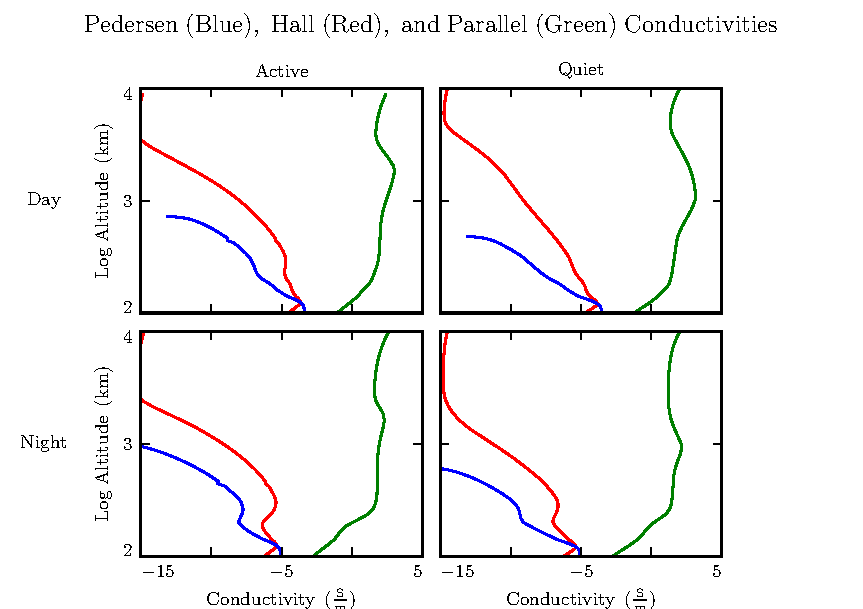
\includegraphics[width=\textwidth]{figures/sigma.pdf}
    \caption[Ionospheric Conductivity Profiles]{
      Ionospheric conductivity profiles, adapted by Lysak\cite{lysak_2013} from Appendix B of Kelley's textbook\cite{kelley_1989}. 
    }
    \label{fig_sigma}
\end{figure}

\todo{What is the height-interated conductivity for each profile? }

% -----------------------------------------------------------------------------
% -----------------------------------------------------------------------------
% -----------------------------------------------------------------------------
\subsection{\Alfven Speed}

The \Alfven speed is computed from Kelley's low-density profile, modified to take into account the local density. The density, in turn, is the sum of a plasmaspheric profile and a high-latitude auroral profile. 
\begin{align}
  \ep &= \text{(low-density tabulated value)} + \frac{ n \bar{m} }{B_0^2}
\end{align}

\todo{What's a clean way of showing the low-density \ep that we read in? }

\todo{Above the profile, Bob scales the value that's read in as $r^5$ or something. Is there a citation for that? }

Where $\bar{m}$ is the ambient mean molecular mass and $B_0$ is the zeroth-order magnetic field strength, $B_0 = \SI{3.11e4}{\nano\tesla} \lr{ \frac{R_E}{r} }^3 \sqrt{ 1 + 3 \cos^2 \theta }$. Note that \SI{3.11e4}{\nano\tesla} is the value of the Earth's magnetic field at the equator on Earth's surface. 

\todo{Cite this number? }

Note that we do not scale the electric constant to units of $\ez$. 

The \Alfven speed is then computed per \cref{def_basics}, $\va^2 \equiv \frac{1}{\mz \ep}$. 

\todo{Put up a plot of the four \Alfven speed profiles. Show the dipole, or zoom in on the ionosphere? }

\todo{Shouldn't the \Alfven speed profiles be brought up early on, since they're necessary for discussions about evanescence at large \azm in \cref{ch_math}? }

\todo{Explain in this section how we figure out the time step. }

% =============================================================================
% =============================================================================
% =============================================================================
\section{Maxwell's Equations}
  \label{sec_eqns}

The model simulates the evolution of electric and magnetic fields in accordance with Maxwell's equations. Specifically, magnetic fields are advanced using \farlaw, and electric fields with \amplaw. Kirchhoff's formulation of \ohmlaw ($\vec{J} = \tensor{\sigma} \cdot \vec{E}$) is used to eliminate the explicit current dependence in \amplaw. 
\begin{align}
  \label{def_eqns}
  \ddt \vec{B} &= - \curl{E} &
  \tensor{\epsilon} \cdot \ddt \vec{E} &= \frac{1}{\mu_0} \curl{B} - \tensor{\sigma} \cdot \vec{E}
\end{align}

% -----------------------------------------------------------------------------
% -----------------------------------------------------------------------------
% -----------------------------------------------------------------------------
\subsection{Notation and Optimization}

Algebra is carried out on paper, producing expressions where each field value is a linear combination of previous field values. These coefficients are computed before the main loop begins. This offers a significant reduction in floating point operations each iteration. 

The \assign operator is used to indicate assignment, rather than equality. Values on the left are new, and those on the right are old. New and old magnetic field values are offset by \dt; electric field values staggered by $\frac{\dt}{2}$. As an example of this notation, \cref{def_assign} integrates \farlaw over a time step, assuming that the curl of the electric field varies slowly compared to \dt: 
\begin{align}
  \label{def_assign}
  \begin{split}
  \int_0^{\dt} dt \, \ddt \vec{B} &= - \displaystyle\int_0^{\dt} dt \, \curl{E} \\ 
  \left. \vec{B} \right|_{\dt} - \left. \vec{B} \right|_0 &= \left. - \dt \, \curl{E} \right|_{ \frac{\dt}{2} } \\
  \vec{B} &\assign \vec{B} - \dt \, \curl{E}
  \end{split}
\end{align}

It's also beneficial to store the curl of each field, rather than take derivatives on the fly. The following sections make use of the shorthand $\vec{C} \equiv \curl{E}$ and $\vec{F} \equiv \curl{B}$. Or, recalling \cref{jacobian_usage}, 
\begin{align}
  \label{def_curls}
  C^i & = \frac{ \varepsilon^{ijk} }{\jac} \dd{\lysakj} E_k &
  F^i & = \frac{ \varepsilon^{ijk} }{\jac} \dd{\lysakj} B_k
\end{align}

Only covariant field components are stored. Only contravariant curl components are stored. This cuts down on memory use, while also eliminating the time spent rotating between bases; those operations are built into the precomputed coefficients. 

% -----------------------------------------------------------------------------
% -----------------------------------------------------------------------------
% -----------------------------------------------------------------------------
\subsection{Magnetic Fields}

Taking advantage of the shorthand defined in \cref{def_curls}, \farlaw is simply written
\begin{align}
  \label{farlaw_ijk}
  \ddt B^i &= - C^i
\end{align}

Or, using the metric tensor to cast the magnetic field in terms of its covariant components, and writing out each coefficient explicitly,
\begin{align}
  \begin{split}
  B_1 &\assign B_1 - g_{11} \, \dt \, C^1 - g_{13} \, \dt \, C^3 \\
  B_2 &\assign B_2 - g_{22} \, \dt \, C^2 \\
  B_3 &\assign B_3 - g_{31} \, \dt \, C^1 - g_{33} \, \dt \, C^3
  \end{split}
\end{align}


% -----------------------------------------------------------------------------
% -----------------------------------------------------------------------------
% -----------------------------------------------------------------------------
\subsection{Electric Fields}
  \label{sec_e}

\amplaw, can be solved with integrating factors. From \cref{def_eqns}, 
\begin{align}
  \tensor{\epsilon} \cdot \ddt \vec{E} &= \frac{1}{\mu_0} \curl{B} - \tensor{\sigma} \cdot \vec{E}
\end{align}

The permittivity tensor is diagonal, and so can be trivially inverted. 
\begin{align}
  \label{amp_tensor}
  \lr{ \tensor{\Omega} + \tensor{ \mathbb{I} } \ddt } \cdot \vec{E} &= \tensor{v}^2 \cdot \vec{F}
\end{align}

Where $\tensor{ \mathbb{I} }$ is the identity tensor and in \x-\y-\z coordinates, 
\begin{align}
  \tensor{v}^2 &\equiv \frac{1}{\mz} \tensor{\epsilon}^{-1} = 
    \mmm{\va^2}{0}{0}
        {0}{\va^2}{0}
        {0}{0}{c^2}
  && \text{and} &
  \tensor{\Omega} &\equiv \tensor{\epsilon}^{-1} \cdot \tensor{\sigma} = 
    \mmm{ \frac{\sp}{\ep} }{ -\frac{\sh}{\ep} }{0}
        { \frac{\sh}{\ep} }{ \frac{\sp}{\ep} }{0}
        {0}{0}{ \frac{\sz}{\ez} } 
\end{align}

Using integrating factors, \cref{amp_tensor} gives
\begin{align}
  \vec{E} &\assign \exp \arg{ -\tensor{\Omega} \; \dt } \cdot \vec{E} + \dt \, \tensor{v}^2 \cdot \exp \arg{ -\tensor{\Omega} \; \tfrac{\dt}{2} } \cdot \vec{F}
\end{align}

\todo{Do we need to be careful here about the difference between a matrix and a tensor? }

The tensor exponential can be evaluated by considering the diagonal and off-diagonal terms separately. 
\begin{align}
  \tensor{\Omega} &= \tensor{\Omega}'
    + \frac{\sh}{\ep} 
    \mmm{0}{-1}{0}
        {1}{0}{0}
        {0}{0}{0} && \text{where} &
  \tensor{\Omega}' &=
    \mmm{ \frac{\sp}{\ep} }{0}{0}
        {0}{ \frac{\sp}{\ep} }{0}
        {0}{0}{ \frac{\sz}{\ez} }
\end{align}

Note that tensors are remarkably well-behaved when exponentiated\cite{hall_2015}, particularly since $\tensor{\Omega}'$ is diagonal, and thus they commute. 
\begin{align}
  \exp \arg{ \tensor{T} } &= \displaystyle\sum_n \frac{1}{ n! } \tensor{T}^n && \text{and} & \exp \arg{ \tensor{T} + \tensor{T}' } &= \exp \arg{ \tensor{T} } \exp \arg{ \tensor{T}' }
\end{align}

The off-diagonal terms collapse into sines and cosines, indicating a rotation about \z. 
\begin{align}
  \label{amp_final}
  \vec{E} &\assign \exp \arg{ -\tensor{\Omega}' \; \dt } \cdot \tensor{R}_z \arg{ \tfrac{-\sh \dt}{\ep} } \cdot \vec{E}
   + \dt \, \tensor{v}^2 \cdot \exp \arg{ -\tensor{\Omega}' \; \tfrac{\dt}{2} } \cdot \tensor{R}_z \arg{ \tfrac{-\sh \dt}{2 \ep} } \cdot \vec{F}
\end{align}

Where 
\begin{align}
  \tensor{R}_z \arg{\theta} &= 
  \mmm{\cos\theta}{-\sin\theta}{0}
      {\sin\theta}{\cos\theta}{0}
      {0}{0}{1}
\end{align}

The parallel term of term of \cref{amp_final} is simply
\begin{align}
  E_\parallel \assign E_\parallel \exp \arg{ \tfrac{- \sz \dt}{\ez} } + c^2 \dt F_\parallel \exp \arg{ \tfrac{- \sz \dt}{2 \ez} }
\end{align}

Or, in covariant terms, 
\begin{align}
  \label{amp_para}
  E_3 \assign E_3 \exp \arg{ \tfrac{- \sz \dt}{\ez} } + c^2 \dt \lr{ g_{31} F^1 + g_{33} F^3 } \exp \arg{ \tfrac{- \sz \dt}{2 \ez} }
\end{align}

For the ionospheric profiles and time steps employed by this model, $\frac{\sz \dt}{\ez}$ is never smaller than $10^3$. As a result, $\exp \arg{ \frac{- \sz \dt}{\ez} }$ is far too small to be stored in a double precision variable. That is, this simulation takes $E_\parallel$ (and, equally, $E_3$) to be uniformly zero. 

This, obviously, precludes any discussion of parallel electric fields or parallel currents. These topics are revisited in \cref{ch_inertia}. 

Not unrelatedly, recalling the definition of the plasma frequency and parallel conductivity from \cref{def_basics}, $\frac{\sz}{\ez}$ can also be written $\frac{\op^2}{\nu}$. 

The plasma frequency is very fast. 

The perpendicular components of \cref{amp_final}, mapped from the physical basis to the contravariant basis (per \cref{def_xyz_directions}) to the covariant basis (per \cref{metric_usage}), give
\begin{alignat}{6}
  \label{e1_final}
  & E_1 + \frac{ g^{13} }{ g^{11} } && E_3 \assign &&   && E_1 && \cos \arg{ \tfrac{- \sh \dt}{\ep} } \exp \arg{ \tfrac{- \sp \dt}{\ep} } &&  \notag \\
  &                                 &&             && + && E_2 && \sin \arg{ \tfrac{- \sh \dt}{\ep} } \exp \arg{ \tfrac{- \sp \dt}{\ep} } &&  \sqrt{ \frac{ g^{22} }{ g^{11} } } \notag \\
  &                                 &&             && + && E_3 && \cos \arg{ \tfrac{- \sh \dt}{\ep} } \exp \arg{ \tfrac{- \sp \dt}{\ep} } &&  \frac{ g^{13} }{ g^{11} } \\
  &                                 &&             && + && F^1 && \cos \arg{ \tfrac{- \sh \dt}{2\ep} } \exp \arg{ \tfrac{- \sp \dt}{2\ep} } &&  \frac{\va^2 \dt}{ g^{11} } \notag \\
  &                                 &&             && + && F^2 && \sin \arg{ \tfrac{- \sh \dt}{2\ep} } \exp \arg{ \tfrac{- \sp \dt}{2\ep} } &&  \frac{\va^2 \dt}{ \sqrt{ g^{11} g^{22} } } \notag \\
  \intertext{and}
  \label{e2_final}
  & && E_2 \assign && - && E_1 && \sin \arg{ \tfrac{- \sh \dt}{\ep} } \exp \arg{ \tfrac{- \sp \dt}{\ep} } &&  \sqrt{ \frac{ g^{11} }{ g^{22} } } \notag \\
  & &&             && + && E_2 && \cos \arg{ \tfrac{- \sh \dt}{\ep} } \exp \arg{ \tfrac{- \sp \dt}{\ep} } &&  \notag \\
  & &&             && - && E_3 && \sin \arg{ \tfrac{- \sh \dt}{\ep} } \exp \arg{ \tfrac{- \sp \dt}{\ep} } &&  \frac{ g^{13} }{ \sqrt{ g^{11} g^{22} } } \\
  & &&             && - && F^1 && \sin \arg{ \tfrac{- \sh \dt}{2\ep} } \exp \arg{ \tfrac{- \sp \dt}{2\ep} } &&  \frac{\va^2 \dt}{ \sqrt{ g^{11} g^{22} } } \notag \\
  & &&             && + && F^2 && \cos \arg{ \tfrac{- \sh \dt}{2\ep} } \exp \arg{ \tfrac{- \sp \dt}{2\ep} } &&  \frac{\va^2 \dt}{ g^{22} } \notag
\end{alignat}

The $E_3$ terms can be ignored at present, but \cref{ch_inertia} references back to them. 

% =============================================================================
% =============================================================================
% =============================================================================
\section{Driving}
  \label{sec_driving}

If no energy is added, the simulation is pretty boring. Everything just stays zero. 

% -----------------------------------------------------------------------------
% -----------------------------------------------------------------------------
% -----------------------------------------------------------------------------
\subsection{Outer Boundary Compression}

Driving from the outer boundary is the traditional way to do it. 

\todo{Cite and briefly explain past work done with compressional driving. This is what most of Bob's papers are, right? }

As discussed in \cref{sec_math_implications}, \Alfven waves become guided when the azimuthal modenumber is large. The energy all stays close to the outer boundary. No field line resonances of significant strength are created within the magnetosphere. 

\todo{Show a plot of compressional driving, maybe day and night, as \azm increases. Mean energy density over time? Something that shows the recession of waves away from the middle of the simulation. }

Compressional driving is applied by setting the value of $B_3$ at the outer boundary. 

A compression might reasonably be expected to drive waves with long azimuthal wavelengths. However, there is some indication that waves with short azimuthal wavelength can be driven as well, such as through Kelvin-Helmholtz interactions. 

\todo{Find this claim again and cite it. }

% -----------------------------------------------------------------------------
% -----------------------------------------------------------------------------
% -----------------------------------------------------------------------------
\subsection{Ring Current Modulation}

Pc4 pulsations with high azimuthal modenumber are known to be driven from within the magnetosphere, such as through drift-resonant interactions with energetic radiation belt and ring current particles. 

\todo{Cite. }

Substorm injection can cause localized ring current behavior. 

\todo{UNH was looking at this at AGU. Check if they have published yet. }

During geomagnetically active times, the ring current is a dynamic region. It's easy to imagine localized perturbations. 

It's difficult to estimate how large such perturbations might be. The following is a kludgey estimate. 

\todo{Plot of Sym-H and its Fourier modes. 1 June 2013. 17 March 2015. 22 June 2015. 17 March 2013. Fit at the ``top'' of the $\frac{1}{f}$ noise. (``Pink noise''?) }

Sym-H is like Dst, but with greater time resolution. 

The noise suggests that a Fourier component with a period of about \SI{1}{\minute} could have an amplitude around \SI{e-3}{\nano\tesla}. 

If the driving is delivered at $L=5$, with a standard deviation of \SI{0.5}{\RE} in the radial direction and \SI{5}{\degree} angularly, that corresponds to a current density of about \SI{4e-4}{\uA/\meter\squared}. This comes from approximating the ring current as a ring of current. Of course, Sym-H is measured at Earth's surface, not at the center of the ring; this gives a geometric factor of about two. 

\todo{What electric field magnitude does this correspond to? }

Current driving is applied by adding an additional current term. \amplaw becomes
\begin{align}
  \tensor{\epsilon} \cdot \ddt \vec{E} &= \frac{1}{\mu_0} \curl{B} - \tensor{\sigma} \cdot \vec{E} - \vec{J}_{drive}
\end{align}

And this driving term is absorbed into the curl by revising \cref{def_curls} from $\vec{F} \equiv \curl{B}$ to $\vec{F} \equiv \curl{B} - \vec{J}_{drive}$. (As a result, \cref{e1_final,e2_final} do not change.)

Notably, Sym-H is a global quantity; it's not ideally suited for making estimates of localized inhomogeneity. 

Furthermore, Sym-H has a time resolution of \SI{1}{\minute}. It can hardly be said to carry information about oscillations at frequencies of less than two minutes. 

Sym-H gives no way to estimate azimuthal modenumber. That's based on Pc4 observations. Dai\cite{dai_2015} observed modenumbers approaching \num{100}. 

A kludgey estimate is better than no estimate. 

% =============================================================================
% =============================================================================
% =============================================================================
\section{Boundary Conditions}
  \label{sec_bcs}

The grid can't go on forever. There have to be special cases at the edges. 


% -----------------------------------------------------------------------------
% -----------------------------------------------------------------------------
% -----------------------------------------------------------------------------
\subsection{Parity and Interpolation}

Computation takes place on a staggered grid. 

Field values are offset to ensure that most differences are centered. For example, $\ddt B_2$ depends on $\dd{\lysakx} E_3$ and $\dd{\lysakz} E_1$. If $B_2$ is defined at even $i$, $E_3$ is defined at odd $i$, so that $B_2$ is defined on the same grid points as $\frac{ E_3 \lrb{i+1} - E_3 \lrb{i-1} }{ \lysakx \lrb{i+1} - \lysakx \lrb{i-1} }$. 

\todo{Make sure the example uses the currect parities. }

\todo{Find a citation for the wigglies that occur if field values are defined on all grid points, due to the weak coupling. This problem is apparently well-known. }

Values are sometimes needed off-parity. $E_1$ and $E_2$ are not defined at the same grid locations, but they are coupled directly by the Hall conductivity. And $B_1$ and $B_3$ are coupled by the non-orthogonality of the grid. When off-parity values are needed, they are interpolated from their neighbors. 

Differentiation and interpolation are good to second order on the nonuniform grid. Like the coefficients for Maxwell's equations, differentiation and interpolation weights are computed during setup to save time during iteration. 

Electric fields go to zero at the innermost and outermost field lines (Dirichlet boundary conditions). Magnetic fields have zero derivative (Neumann boundary conditions). For components not defined at the exact boundary, these rules are applied when differentiating or interpolating; they set the effective value just outside the grid. 

These boundary conditions can in principle cause nonphysical reflection at the boundary. In practice, that is not an issue. Wave activity is concentrated well away from the boundaries. In fact, reversing the Dirichlet and Neumann boundary conditions has little effect. 

(Of course, an inconsistent boundary condition -- like using the same boundary condition for a field and its derivative -- causes instability.)

% -----------------------------------------------------------------------------
% -----------------------------------------------------------------------------
% -----------------------------------------------------------------------------
\subsection{Coupling to the Atmosphere}

Conditions at the ionospheric boundaries are set by coupling to the atmosphere. This also allows the computation of ground fields. 

It's reasonable to approximate the atmosphere as a perfect insulator, giving $\curl{B}=0$. Combining with $\div{B}=0$ per Maxwell's equations, ensures the existence of a scalar magnetic potential $\Psi$ such that $\vec{B}=\grad{\Psi}$ and $\Psi$ satisfies Laplace's equation, $\nabla^2 \Psi = 0$. 

Laplace's equation can be solved analytically; in spherical coordinates, the solutions are spherical harmonics. However, a numerical solution is preferrable to ensure orthonormality on a discrete (and incomplete -- there are no grid points at the poles or equator) grid. After separating out the radial and azimuthal dependence in the usual way, the latitudinal component of Laplace's equation (in terms of $s \equiv - \sin^2 \theta$) is
\begin{align}
  \label{laplace}
  \lr{ 4 s^2 + 4s } \frac{d^2}{ds^2} Y_\ell + \lr{ 4 + 6 s } \frac{d}{ds} Y_\ell - \frac{\azm^2}{s} Y_\ell &= \ell \lr{ \ell + 1 } Y_\ell
\end{align}

Using centered differences to express the derivatives, \cref{laplace} is a system of linear equations, one per field line. It can be solved numerically for eigenvalues $\ell \lr{\ell + 1}$ and eigenvectors (harmonics) $Y_\ell$. In terms of those harmonics, and noting that the model uses a fixed azimuthal modenumber \azm, $\Psi$ between $R_E$ and $R_I$ can be expressed
\begin{align}
  \label{psi_expansion}
  \Psi \arg{r, \theta, \phi} &= \displaystyle\sum_\ell \lr{ \alpha_\ell \, r^\ell + \beta_\ell \, r^{-\ell - 1} } Y_\ell \arg{\theta} \exp \arg{i \azm \phi}
\end{align}

As a boundary condition for $\Psi$, Earth's crust is assumed to be a perfect conductor, forcing the magnetic field at the boundary to be perfectly horizontal. That is, $B_r = \dd{r} \Psi = 0$. Then, noting that the harmonics $Y_\ell$ are orthonormal (so each term of the sum must be zero), 
\begin{align}
  \label{beta_solution}
  \beta_\ell &= \frac{\ell}{\ell + 1} R_E^{2 \ell + 1} \alpha_\ell
\end{align}

Note that the explicit $\phi$ dependence has been dropped. The entire simulation shares a fixed modenumber, so it's sufficient to find $\Psi$ at $\phi=0$. 

At the top of the atmosphere, the radial magnetic field is again used as a boundary condition, this time to compute the weights $\alpha_\ell$. 

\todo{Something something thin horizontal current sheet at $R_I$. }

Taking the shorthand $\lambda_I \equiv \frac{R_E}{R_I} \sim \num{0.975}$
\begin{align}
  B_r &= \displaystyle\sum_\ell \ell \, \alpha_\ell \, R_I^{\ell-1} \, \lr{ 1 - \lambda_I^{2 \ell - 1} } Y_\ell
\end{align}

\todo{Settle on good notation for taking the inner product of harmonics. It's a vector in the sense that it's a one-dimensional array of values, but not in the physical sense. Indexing -- $B_r\lrb{i}$ -- also seems awkward. }

The sum can be collapsed by ``integrating" over a harmonic. The inverse harmonics are obtained by inverting the eigenvector matrix. Then $Y_\ell \cdot Y_{\ell'}^{-1} = \delta_{\ell \ell'}$ by construction. 
\begin{align}
  \label{alpha_solution}
  \alpha_\ell &= \frac{ 1 }{\ell \, R_I^{\ell-1} } \frac{ B_r \cdot Y_\ell^{-1} }{ 1 + \lambda_I^{2 \ell + 1} }
\end{align}

Combining \cref{psi_expansion,beta_solution,alpha_solution} allows the expression of $\Psi$ at the top and bottom of the atmosphere as a linear function of the radial magnetic field at the boundary. 
\begin{align}
  \label{psi_final}
  \begin{split}
  \Psi_E &= \displaystyle\sum_\ell Y_\ell \; \frac{R_I}{\ell} \frac{ \frac{2 \ell - 1}{\ell - 1} \lambda^\ell }{ 1 - \lambda_I^{2 \ell + 1} } B_r \cdot Y_\ell^{-1} \\
  \Psi_I &= \displaystyle\sum_\ell Y_\ell \; \frac{R_I}{\ell} \frac{ 1 + \frac{\ell}{\ell - 1} \lambda_I^{2 \ell + 1} }{ 1 - \lambda_I^{2 \ell + 1} } B_r \cdot Y_\ell^{-1}
  \end{split}
\end{align}

Magnetic fields are evaluated from $\Psi$ per 
\begin{align}
  B_1 &= \dd{\lysakx} \Psi &
  B_2 &= \dd{\lysaky} \Psi
\end{align}

Note that $B_1$ and $B_2$ are horizontal; per \cref{def_rqf_directions}, they are proportional to $B_\theta$ and $B_\phi$ respectively. 

At the ground, field values are purely output. 

Horizontal magnetic field values at the top of the ionosphere, on the other hand, are used as boundary conditions. Assuming there is no vertical component to the ionospheric current sheet, the electric field values at the ionospheric edge of the grid are dictated by the jump in horizontal magnetic field between the bottom of the grid and the top of the atmosphere. 
\begin{align}
  \mz \, \tensor{\Sigma} \cdot \vec{E} &= \left. \displaystyle\lim_{\dr \rightarrow 0} \, \hat{r} \! \times \! \vec{B} \, \right|^{R_I + \dr}_{R_I - \dr}
\end{align}

\todo{Bob's citations for the ionospheric jump conditions: Fujita and Tamao 1988, Yosikawa and Itonaga 1996, 2000, Lysak and Song 2001, Sciffer and Waters 2002. It basically comes from integrating \amplaw, so half a dozen citations seems like overkill. }




% %%%%%%%%%%%%%%%%%%%%%%%%%%%%%%%%%%%%%%%%%%%%%%%%%%%%%%%%%%%%%%%%%%%%%%%%%%%%%
% %%%%%%%%%%%%%%%%%%%%%%%%%%%%%%%%%%%% Compute the Dispersion Relation for Tuna
% %%%%%%%%%%%%%%%%%%%%%%%%%%%%%%%%%%%%%%%%%%%%%%%%%%%%%%%%%%%%%%%%%%%%%%%%%%%%%

\chapter{Waves in Cold Resistive Plasmas}
  \label{ch_math}

\todo{Sketch out what a dispersion relation is, why it works, why it's interesting. }

\todo{Explain that the inclusion of conductivity is novel. }

\todo{This chapter works out the sorts of waves that might be expected in the numerical model. It starts with the same equations that are used by the model -- Maxwell's equations and \ohmlaw. The resulting dispersion relation is too high-ordered for a direct solution, so several limits of interest are considered. } 

\section{The Dispersion Tensor}

\todo{At this end of this chapter, there will be a discussion of what is specifically interesting about the findings. That doesn't really exist yet. Or... actually, should we discuss interesting things as we find them? Note that we find $\omega^2 = k^2 \va^2$ several times. }

Cold, linearlized \amplaw and \farlaw. The vector $\vec{B}$ is the perturbation to the zeroth-order magnetic field. 
\begin{align}
  \ddt \vec{B} &= -\curl{E} & \tensor{\epsilon} \cdot \ddt \vec{E} &= \oomz \curl{B} - \vec{J}
\end{align}

\ohmlaw. Electron inertial effects are included in the parallel direction. See \cref{ch_inertia}. 
\begin{align}
  \frac{\me}{n e^2} \ddt J_\parallel & = 
    \sz E_\parallel - J_\parallel &
  0 & = 
    \tensor{\sigma}_\bot \cdot \vec{E}_\bot - \vec{J}_\bot
\end{align}

Suppose that the fields and currents are resonating as $\exp \arg{i \vec{k} \cdot \vec{x} - i \omega t }$. Evaluate the derivatives. Eliminate magnetic fields and currents. 
\begin{alignat}{4}
  \label{disp_para}
  & 0 = E_\parallel && + \frac{c^2}{\omega^2} \lr{ \vec{k} \, \vec{k} \cdot \vec{E} - k^2 \vec{E} }_\parallel && + \frac{i \op^2 }{\omega \lr{\nu - i \omega} } && E_\parallel \\
  \label{disp_perp}
  & 0 = \vec{E}_\bot && + \frac{\va^2}{\omega^2} \lr{ \vec{k} \, \vec{k} \cdot \vec{E} - k^2 \vec{E} }_\bot && + \frac{i}{\ep \omega} \tensor{\sigma}_\bot \cdot && \vec{E}_\bot
\end{alignat}

The above expression makes use of the vector identity $\vec{k} \times \vec{k} \times \vec{E} = \vec{k} \, \vec{k} \cdot \vec{E} - k^2 \vec{E}$. The \Alfven speed, speed of light, plasma frequency, and parallel conductivity are defined in the usual way: 
\begin{align}
  \label{def_basics}
  \va^2 & \equiv \frac{1}{\mz \ep} &
  c^2 & \equiv \frac{1}{\mz \ez} &
  \op^2 & \equiv \frac{n e^2}{\me \ez} &
  \sz & \equiv \frac{n e^2}{\me \nu}
\end{align}

Note that this definition of the \Alfven speed takes into account the displacement current correction which is important when \va approaches $c$. 

Without loss of generality, the wave vector $\vec{k}$ can be said to lie in the \x-\z plane; the distinction between the \x and \y directions is revisited in \cref{sec_math_implications}. Let $\theta$ be the angle between $\vec{k}$ and the zeroth-order magnetic field. 

Then \cref{disp_para,disp_perp} can be combined into the usual dispersion tensor form, $\dispersiontensor \cdot \vec{E} = 0$, where 
\begin{align}
  \dispersiontensor & = \tensor{ \mathbb{I} }
                      + \frac{k^2}{\omega^2} 
                        \mmm{-\va^2 \cos^2 \theta}{0}{\va^2 \sin \theta \cos \theta}
                            {0}{-\va^2}{0}
                            {c^2 \sin \theta \cos \theta}{0}{-c^2 \sin^2 \theta}
                      + \frac{i}{\omega}
                        \mmm{ \frac{\sp}{\ep} }{-\frac{\sh}{\ep} }{0}
                            { \frac{\sh}{\ep} }{ \frac{\sp}{\ep} }{0}
                            {0}{0}{ \frac{\op^2}{\nu - i \omega} }
\end{align}

Nontrivial solutions exist only when $\left| \dispersiontensor \right| = 0$. This gives rise to a seventh-order polynomial in $\omega$, so it's necessary to consider limits of particular interest. 

% =============================================================================
% =============================================================================
% =============================================================================
\section{Parallel Propagation Limit}

Parallel propagation is a naive representation of a field line resonance; the wave vector moves energy along the field line. Taking $\theta=0$, $\dispersiontensor$ simplifies to
\begin{align}
  \label{parallel_dispersion_tensor}
  \dispersiontensor_\parallel & = \tensor{ \mathbb{I} }
                      - \frac{k^2 \va^2}{\omega^2} 
                        \mmm{1}{0}{0}
                            {0}{1}{0}
                            {0}{0}{0}
                      + \frac{i}{\omega}
                        \mmm{ \frac{\sp}{\ep} }{-\frac{\sh}{\ep} }{0}
                            { \frac{\sh}{\ep} }{ \frac{\sp}{\ep} }{0}
                            {0}{0}{ \frac{\op^2}{\nu - i \omega} }
\end{align}

Conveniently, parallel and perpendicular polarizations are not coupled in \cref{parallel_dispersion_tensor}. 

% -----------------------------------------------------------------------------
% -----------------------------------------------------------------------------
% -----------------------------------------------------------------------------
\subsection{Parallel Polarization}

The parallel component of the determinant of \cref{parallel_dispersion_tensor} gives
\begin{align}
  \omega^2 + i \nu \omega - \op^2 = 0
\end{align}

With no $k$ dependence this expression doesn't describe a wave per se, so much as a resonant frequency. Solving directly, 
\begin{align}
  \omega & = -\frac{i \nu}{2} \pm \sqrt{ \op^2 - \frac{\nu^2}{4} }
\end{align}

The plasma frequency significantly exceeds the collision frequency everywhere except a narrow strip at the ionospheric boundary of the model. Expanding in large $\op$ gives
\begin{align}
  \omega^2 & = \op^2 - i \nu \op + ...
\end{align}

\todo{Actually, double-check this. How does $\nu$ compare to $\op$ at the ionospheric boundary when there is no Boris factor? }

This is the plasma oscillation. 

% -----------------------------------------------------------------------------
% -----------------------------------------------------------------------------
% -----------------------------------------------------------------------------
\subsection{Perpendicular Polarization}

The perpendicular components of the determinant of \cref{parallel_dispersion_tensor} give
\begin{align}
  \omega^4 + 2 i \frac{\sp}{\ep} \omega^3
  - \lr{ 2 k^2 \va^2 + \frac{\sp^2 + \sh^2}{\ep^2} } \omega^2
  - 2 i k^2 \va^2 \frac{\sp}{\ep} \omega
  + k^4 \va^4 & = 0
\end{align}

This can be solved in exact form. Noting that $\pm$ and $\opm$ are independent,
\begin{align}
  \omega = \lr{ \frac{\pm \sh - i \sp}{2 \ep} } \opm \sqrt{ k^2 \va^2 + \lr{ \frac{\pm \sh - i \sp}{2 \ep} }^2 }
\end{align}

Over the vast majority of a field line, $k \va \gg \frac{\sp}{\ep}$ and $k \va \gg \frac{\sh}{\ep}$. 
\begin{align}
  \omega^2 = k^2 \va^2 \opm k \va \frac{\sh \pm i \sp}{\ep} + ...
\end{align}

This is the \Alfven wave, evidently split by the ionospheric conductivity, propagating along the zeroth-order magnetic field line. 

% =============================================================================
% =============================================================================
% =============================================================================
\section{Perpendicular Propagation Limit}

A wave's ability to propagate across field lines is also of interest. When $\theta = \frac{\pi}{2}$, $\dispersiontensor$ simplifies to
\begin{align}
  \label{perp_dispersion_tensor}
  \dispersiontensor_\bot & = \tensor{ \mathbb{I} }
                      - \frac{k^2}{\omega^2} 
                        \mmm{0}{0}{0}
                            {0}{\va^2}{0}
                            {0}{0}{c^2}
                      + \frac{i}{\omega}
                        \mmm{ \frac{\sp}{\ep} }{-\frac{\sh}{\ep} }{0}
                            { \frac{\sh}{\ep} }{ \frac{\sp}{\ep} }{0}
                            {0}{0}{ \frac{\op^2}{\nu - i \omega} }
\end{align}

As in the parallel propagation case, the parallel and perpendicular components of the determinant are decoupled. 

% -----------------------------------------------------------------------------
% -----------------------------------------------------------------------------
% -----------------------------------------------------------------------------
\subsection{Parallel Polarization}

The parallel component of the determinant of \cref{perp_dispersion_tensor} gives
\begin{align}
  \omega^3 + i \nu \omega^2
  - \lr{ k^2 c^2 + \op^2 } \omega
  - i k^2 c^2 \nu & = 0
\end{align}

The above expression can be solved exactly, but the resulting expressions are too long to be useful. 

Expanding the solution in large $\op$ gives the O mode: a compressional wave with a parallel electric field. 
\begin{align}
  \omega^2 & = k^2 c^2 + \op^2 - i \nu \op + ...
\end{align}


% -----------------------------------------------------------------------------
% -----------------------------------------------------------------------------
% -----------------------------------------------------------------------------
\subsection{Perpendicular Polarization}

The perpendicular components of the determinant of \cref{perp_dispersion_tensor} give
\begin{align}
  \omega^3 + 2 i \frac{\sp}{\ep} \omega^2
  - \lr{ 2 k^2 \va^2 + \frac{\sp^2 + \sh^2}{\ep^2} } \omega
   - i k^2 \va^2 \frac{\sp}{\ep} & = 0
\end{align}

Again, the roots of the cubic are impractically long. 

Expanding in large conductivity, as is expected near the ionospheric boundary, gives
\begin{align}
  \omega^2 & = k^2 \va^2 + \lr{ \frac{\sh \pm i \sp}{\ep} }^2 + ...
\intertext{Whereas expanding in small conductivity, as is expected far from the boundary, gives}
  \omega^2 & = k^2 \va^2 \pm i k \va \frac{\sp}{\ep} + ...
\end{align}

Both of which are \Alfven waves. 

% =============================================================================
% =============================================================================
% =============================================================================
\section{High Altitude Limit}
  \label{sec_high_alt}

At high altitude, where the density is very low compared to the ionosphere, it's reasonable to approximate $\sp \rightarrow 0$ and $\sh \rightarrow 0$ and $\nu \rightarrow 0$. 

In this case, $\dispersiontensor$ simplifies to

\begin{align}
  \label{high_dispersion_tensor}
  \dispersiontensor_{\infty} & = \tensor{ \mathbb{I} }
                      - \frac{k^2}{\omega^2} 
                        \mmm{\va^2 \cos^2 \theta}{0}{-\va^2 \sin \theta \cos \theta}
                            {0}{\va^2}{0}
                            {-c^2 \sin \theta \cos \theta}{0}{c^2 \sin^2 \theta}
                      - \frac{\op^2}{\omega^2}
                        \mmm{0}{0}{0}
                            {0}{0}{0}
                            {0}{0}{1}
\end{align}

In this case it's the azimuthal polarization that decouples from the other two. 

% -----------------------------------------------------------------------------
% -----------------------------------------------------------------------------
% -----------------------------------------------------------------------------
\subsection{Azimuthal Polarization}

The azimuthal component of the determinant of \cref{high_dispersion_tensor} simply gives the \Alfven wave. 
\begin{align}
  \omega^2 & = k^2 \va^2
\end{align}

% -----------------------------------------------------------------------------
% -----------------------------------------------------------------------------
% -----------------------------------------------------------------------------
\subsection{Meridional Polarization}

The components of the determinant of \cref{high_dispersion_tensor} which fall in the meridional plane give, taking $k_\bot \equiv k \sin \theta$ and $k_\parallel \equiv k \cos \theta$,
\begin{align}
  \omega^4 
  - \lr{ k_\parallel^2 \va^2 + k_\bot^2 c^2 + \op^2 } \omega^2
  + k_\parallel^2 \va^2 \op^2  & = 0
\end{align}

The above expression is quadratic in $\omega^2$, and thus can be solved directly. 
\begin{align}
  \omega^2 & = \frac{1}{2} \lr{ k_\parallel^2 \va^2 + k_\bot^2 c^2 + \op^2 }
  \pm \sqrt{ \frac{1}{4} \lr{ k_\parallel^2 \va^2 + k_\bot^2 c^2 + \op^2 }^2 
    - k_\parallel^2 \va^2 \op^2 }
\end{align}

Noting that $\op$ is very large, the two roots simplify to
\begin{align}
  \label{high_alt_final}
  \begin{split}
  \omega^2 & = k_\parallel^2 \va^2 + ... \\
  \omega^2 & = k_\parallel^2 \va^2 + k_\bot^2 c^2 + \op^2 + ...
  \end{split}
\end{align}

% =============================================================================
% =============================================================================
% =============================================================================
\section{Implications for This Work}
  \label{sec_math_implications}

% -----------------------------------------------------------------------------
% -----------------------------------------------------------------------------
% -----------------------------------------------------------------------------
\subsection{Mode Coupling}

\todo{Have we got enough/appropriate math here to talk about how $\sh$ rotates fields at the ionosphere? Doubtful. }

% -----------------------------------------------------------------------------
% -----------------------------------------------------------------------------
% -----------------------------------------------------------------------------
\subsection{High Modenumber Cutoff}

As $\azm$ becomes large, it puts a lower bound on the modenumber, and thus on the frequency. For an \Alfven wave, $\omega^2 = k^2 \va^2$,
\begin{align}
  k \ge k_\phi = \frac{\azm}{2 \pi r} \qquad \text{so} \qquad \omega \ge \frac{\azm}{2 \pi r} \va
\end{align}

Any wave with a frequency below this threshold will become evanescent. 

\todo{This point is pretty important. It's revisited in \cref{sec_driving}. }




% %%%%%%%%%%%%%%%%%%%%%%%%%%%%%%%%%%%%%%%%%%%%%%%%%%%%%%%%%%%%%%%%%%%%%%%%%%%%%
% %%%%%%%%%%%%%%%%%%%%%%%%%%%%%%%%%%%%%%%%%%%%%%%%%% Results of Numerical Model
% %%%%%%%%%%%%%%%%%%%%%%%%%%%%%%%%%%%%%%%%%%%%%%%%%%%%%%%%%%%%%%%%%%%%%%%%%%%%%

\chapter{Results from Numerical Model}
\label{results_chapter}

\section{Azimuthal Poloidal/Toroidal Dichotomy}

This is novel...





% %%%%%%%%%%%%%%%%%%%%%%%%%%%%%%%%%%%%%%%%%%%%%%%%%%%%%%%%%%%%%%%%%%%%%%%%%%%%%
% %%%%%%%%%%%%%%%%%%%%%%%%%%%%%%%%%%%%%%%%%%%%%%%%% Comparison of Model to Data
% %%%%%%%%%%%%%%%%%%%%%%%%%%%%%%%%%%%%%%%%%%%%%%%%%%%%%%%%%%%%%%%%%%%%%%%%%%%%%

\chapter{Comparison to Data}
\label{data_chapter}

GOES, Polar. Look at resources from GEM. 


Case studies! 





% %%%%%%%%%%%%%%%%%%%%%%%%%%%%%%%%%%%%%%%%%%%%%%%%%%%%%%%%%%%%%%%%%%%%%%%%%%%%%
% %%%%%%%%%%%%%%%%%%%%%%%%%%%%%%%%%%%%%%%%%%%%%%%%%% Results of Numerical Model
% %%%%%%%%%%%%%%%%%%%%%%%%%%%%%%%%%%%%%%%%%%%%%%%%%%%%%%%%%%%%%%%%%%%%%%%%%%%%%

\chapter{Giant Pulsations}
\label{giant_pulations_chapter}

\section{something}

This is novel...








\chapter{Conclusion}
  \label{ch_conclusion}


% -----------------------------------------------------------------------------
% -----------------------------------------------------------------------------
% -----------------------------------------------------------------------------
\section{Summary of Results}

\todo{Write this. }


% -----------------------------------------------------------------------------
% -----------------------------------------------------------------------------
% -----------------------------------------------------------------------------
\section{Future Work}

Arbitrary deformation of grid. Get $\hat{e}_i = \frac{\partial}{\partial u^i} \underline{x}$, then $g_{ij} = \hat{e}_i \cdot \hat{e}_j$, then invert the metric tensor for contravariant components.  

MPI. Some benchmarks with time to compute vs time to broadcast. At what problem scale does additional parallelization make sense? 

Driving based on events? Wouldn't be that hard. 

Test particles? Seems silly. Watching something drift-bounce resonate will require making assumptions about what's going on on the other face of the planet.  

Conductivity affected by precipitation/current? 

IRI ionosphere model. Solar illumination effects. 


% Bibliography
\bibliography{thesis}

% Appendices
\appendix

%%%%%%%%%%%%%%%%%%%%%%%%%%%%%%%%%%%%%%%%%%%%%%%%%%%%%%%%%%%%%%%%%%%%%%%%%%%%%%%%
% app_glossary.tex: Glossary Appendix:
%%%%%%%%%%%%%%%%%%%%%%%%%%%%%%%%%%%%%%%%%%%%%%%%%%%%%%%%%%%%%%%%%%%%%%%%%%%%%%%%
\chapter{Glossary and Acronyms}
\label{app_glossary}
%%%%%%%%%%%%%%%%%%%%%%%%%%%%%%%%%%%%%%%%%%%%%%%%%%%%%%%%%%%%%%%%%%%%%%%%%%%%%%%%
Care has been taken in this thesis to minimize the use of jargon and
acronyms, but this cannot always be achieved.  This appendix defines
jargon terms in a glossary, and contains a table of acronyms and their
meaning.
%%%%%%%%%%%%%%%%%%%%%%%%%%%%%%%%%%%%%%%%%%%%%%%%%%%%%%%%%%%%%%%%%%%%%%%%%%%%%%%%

%%%%%%%%%%%%%%%%%%%%%%%%%%%%%%%%%%%%%%%%%%%%%%%%%%%%%%%%%%%%%%%%%%%%%%%%%%%%%%%%
% Glossary {{{
%%%%%%%%%%%%%%%%%%%%%%%%%%%%%%%%%%%%%%%%%%%%%%%%%%%%%%%%%%%%%%%%%%%%%%%%%%%%%%%%
\section{Glossary}
\label{jargonapp}
%%%%%%%%%%%%%%%%%%%%%%%%%%%%%%%%%%%%%%%%%%%%%%%%%%%%%%%%%%%%%%%%%%%%%%%%%%%%%%%%
\begin{itemize}

\item \textbf{Cosmic-Ray Muon} (\textbf{CR $\mu$}) -- A muon coming from
the abundant energetic particles originating outside of the Earth's
atmosphere.

\end{itemize}
%%%%%%%%%%%%%%%%%%%%%%%%%%%%%%%%%%%%%%%%%%%%%%%%%%%%%%%%%%%%%%%%%%%%%%%%%%%%%}}}

%%%%%%%%%%%%%%%%%%%%%%%%%%%%%%%%%%%%%%%%%%%%%%%%%%%%%%%%%%%%%%%%%%%%%%%%%%%%%%%%
% Acronyms {{{
%%%%%%%%%%%%%%%%%%%%%%%%%%%%%%%%%%%%%%%%%%%%%%%%%%%%%%%%%%%%%%%%%%%%%%%%%%%%%%%%
\section{Acronyms}
\label{acronymsec}
%%%%%%%%%%%%%%%%%%%%%%%%%%%%%%%%%%%%%%%%%%%%%%%%%%%%%%%%%%%%%%%%%%%%%%%%%%%%%%%%

% Table formatting

% Heading for the first page
\begin{longtable}{p{0.25\textwidth} p{0.75\textwidth}}
\caption{Acronyms} \label{tab:acronyms} \\

\toprule
Acronym & Meaning \\
\midrule
\endfirsthead

% Heading for all subsequent pages
\multicolumn{2}{l}{\textit{\tablename\ \thetable{} -- Continued from previous page}} \\
\toprule
Acronym & Meaning \\
\midrule
\endhead

% Footer for each page that wraps over to the next
\multicolumn{2}{r}{\textit{Continued on next page}} \\
\bottomrule
\endfoot

% Footer for the end of the table
\bottomrule
\endlastfoot

% End table formatting

CR$\mu$ & Cosmic-Ray Muon \\

\end{longtable}
%%%%%%%%%%%%%%%%%%%%%%%%%%%%%%%%%%%%%%%%%%%%%%%%%%%%%%%%%%%%%%%%%%%%%%%%%%%%%}}}


% %%%%%%%%%%%%%%%%%%%%%%%%%%%%%%%%%%%%%%%%%%%%%%%%%%%%%%%%%%%%%%%%%%%%%%%%%%%%%
% %%%%%%%%%%%%%%%%%%%%%%%%%%%%%%%%%%%%%%%%%%%%%%% Appendix: Integrating Factors
% %%%%%%%%%%%%%%%%%%%%%%%%%%%%%%%%%%%%%%%%%%%%%%%%%%%%%%%%%%%%%%%%%%%%%%%%%%%%%








\chapter{Integrating Factors}
\label{app_integrating}

Start with differential equation of the form:

\begin{align}
  \frac{\partial}{\partial t} X(t) + \alpha X(t) &= \beta
\end{align}

Multiply by the integrating factor, then group terms: 

\begin{align}
  \exp (\alpha \; t) \frac{\partial}{\partial t} X(t) + \alpha \exp(\alpha \; t) X(t) &= \beta \exp(\alpha \; t) \\
  \frac{\partial}{\partial t} \big[ \exp(\alpha t) X(t) \big] &= \beta \exp(\alpha t)
\end{align}

Integrate from 0 to $\delta t$, assuming that $\beta$ is constant in time or varies slowly. 

\begin{align}
  \int^{\delta t}_0 dt \frac{\partial}{\partial t} \big[ \exp(\alpha t) X(t) \big] &= \int^{\delta t}_0 dt \beta \exp(\alpha t) \\
  \exp (\alpha \dt) X(\dt) - X(0) &= \dt \beta ( \frac{\dt}{2} ) \exp ( \alpha \frac{\dt}{2} )
\end{align}

Then rearrange to solve for the new value of X:

\begin{align}
  X(\delta t) &= X(0) \exp ( -\alpha \delta t ) + \delta t \beta ( \frac{\delta t}{2} ) \exp ( -\alpha \frac{\delta t}{2} )
\end{align}

Done. 


% End the Document
\end{document}




